% Appendix for the semantic control task of \cref{sec:degradation}.
% Input from results.tex, after the localization appendix, so that the appendix
% order follows the order of the Results section.
% Source: results/experiment4/main/summary.json, the per-cell summary of Slurm
% job 8333, joined cell by cell against results/experiment1/full32_all.
% Figures: python code/analysis/plot_paper_figures.py

\section{Task Degradation: Additional Details}
\label{app:degradation}

\subsection{Sweep}
\label{app:deg-design}

% CONSISTENCY NOTE (2026-09-16). Experiment 1 was extended to ten concept and ten
% fixed random directions; this sweep was not, and it imports nothing from it
% (summary.json has experiment1_summary: null -- its detection_accuracy is measured
% here). So no number below is arithmetically stale. Two mismatches remain, both
% understating this sweep's concept row relative to Experiment 1:
%   1. It injects only Dust and Satellites, and Dust carries 3 of the 5 evaluated
%      concepts, i.e. 60% of the concept cells. Dust is 9th of 10 in Experiment 1's
%      alpha panel (S = +0.059 against a panel mean of +0.143), so this sweep's
%      concept axis sits about 33% below the full panel's concept mean.
%   2. Detection here is adjusted accuracy at a 0.70 threshold, the estimator
%      app:loc-bias shows does not remove the answer bias; Experiment 1 reports the
%      paired contrast S for that reason. Mean detection accuracy is 0.536-0.569
%      across families, i.e. the bias-pinned regime.
% Also: this sweep's calibration is the superseded isolated-sentence one and its z
% grid stops at 20.48, so its standardized half is void -- already stated below, and
% every figure filters to matched alpha.
Five concepts of the complex-example corpus are evaluated
(\emph{appreciation}, \emph{betrayal}, \emph{Fibonacci numbers},
\emph{recursion}, \emph{shutdown}), each with four positive and four negative
sentences under both assignments of the letters \texttt{X} and \texttt{Y}: 80
items over 40 distinct sentences. The injected direction, \emph{Dust} or
\emph{Satellites}, is never the evaluated concept. The sweep covers blocks
0--30, the four families, ten raw amplitudes from $0.25$ to $128$ and twelve
standardized doses, for 436,480 perturbed trials against the same 80 sham
trials throughout, with 80 trials per concept cell, 160 for renewed noise and
for dropout and 240 for fixed random, those families carrying two, two, two
and three directions or realizations. Block 31 is excluded: its concept
directions cannot be rebuilt to the norm the calibration recorded, and by
\cref{sec:localization} it is structurally dead in any case.

\subsection{Depth Profile and Matched Degradation}
\label{app:deg-depth}

Blocks 0--7 do not separate the families (\cref{tab:app-deg-depth}): in the
early stack everything breaks the task equally, between $-0.23$ and $-0.36$.
From block 8 the three controls recover and the concept family does not, the
gap peaking at $-0.197$ at block 9: the deepest block whose pooled loss still
reaches 5 points is 9 for renewed noise and for dropout, 10 for fixed random
directions and 15 for concept. Above the contiguous band the concept family
oscillates rather than staying flat, $-0.083$ at block 15 against $0.000$ at
block 16, so isolated deep cells survive that criterion while
\cref{sec:localization} reports the deep localization zero as exact.

\begin{table}[H]
\centering
\small
\begin{tabular}{rrrrrr}
\toprule
Block & Concept & Fixed & Noise & Dropout & Gap \\
\midrule
7  & $-0.272$ & $-0.261$ & $-0.231$ & $-0.245$ & $-0.026$ \\
8  & $-0.295$ & $-0.144$ & $-0.157$ & $-0.152$ & $-0.144$ \\
9  & $-0.298$ & $-0.144$ & $-0.079$ & $-0.080$ & $-0.197$ \\
10 & $-0.103$ & $-0.081$ & $-0.038$ & $-0.031$ & $-0.053$ \\
12 & $-0.119$ & $-0.033$ & $0.000$  & $-0.004$ & $-0.106$ \\
15 & $-0.083$ & $0.014$  & $0.017$  & $0.014$  & $-0.098$ \\
18 & $-0.003$ & $0.010$  & $0.002$  & $0.003$  & $-0.008$ \\
\bottomrule
\end{tabular}
\caption{Classification accuracy minus sham, pooled over the four largest raw
amplitudes. Fixed denotes fixed random directions. Gap is concept minus the
mean of the three controls.}
\label{tab:app-deg-depth}
\end{table}

\Cref{tab:app-deg-matched} bins the cells of both dose rules by accuracy loss
and compares localization within each bin.

\begin{table}[H]
\centering
\small
\begin{tabular}{lrrrr}
\toprule
Accuracy loss & Concept & Fixed & Noise & Dropout \\
\midrule
$[-1.00,-0.30)$ & 0.733 & 0.588 & 0.716 & 0.671 \\
$[-0.30,-0.15)$ & 0.712 & 0.659 & 0.688 & 0.693 \\
$[-0.15,-0.05)$ & 0.658 & 0.643 & 0.709 & 0.718 \\
$[-0.05,+0.05]$ & 0.521 & 0.508 & 0.518 & 0.516 \\
\bottomrule
\end{tabular}
\caption{Mean localization accuracy at matched classification loss, both dose
rules pooled. Doses are pooled inside a bin, so a family that reaches a bin at
a much lower dose than another is not distinguished here.}
\label{tab:app-deg-matched}
\end{table}

\subsection{Maps}
\label{app:deg-maps}

\begin{figure}[htbp]
\centering
\begin{minipage}[t]{0.48\textwidth}
\centering
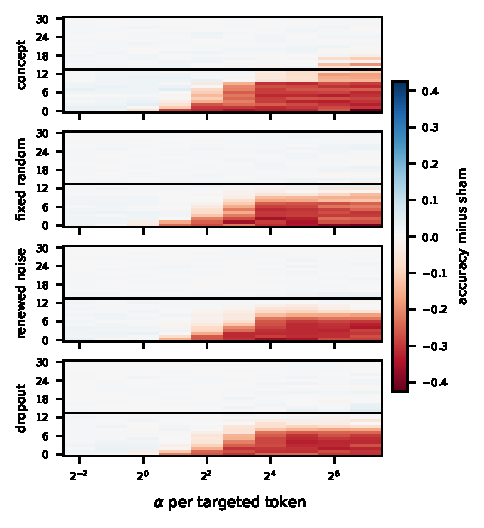
\includegraphics[width=\linewidth]{figures/degradation_maps.pdf}
\end{minipage}\hfill
\begin{minipage}[t]{0.48\textwidth}
\centering
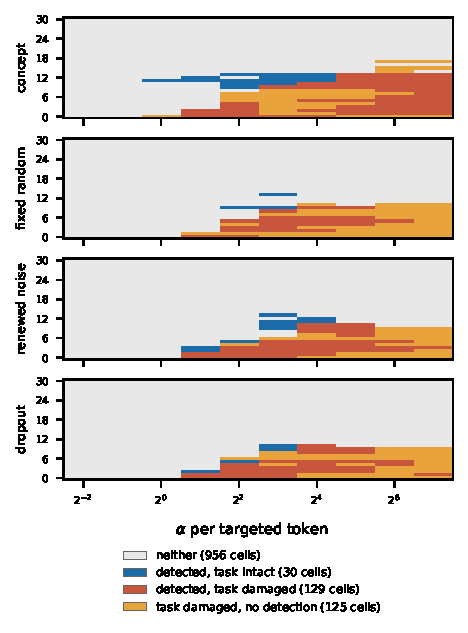
\includegraphics[width=\linewidth]{figures/degradation_regimes.pdf}
\end{minipage}
\caption{Left: classification accuracy minus sham by block and raw amplitude,
one row per family, red for degradation; the rule marks block 14, the first
block above the contiguous degraded band, and the colour scale is symmetric
about zero by construction, so that deep-block noise does not read as vividly
as shallow-block collapse. Right: the joint regimes over the same cells. A
cell counts as detected when the localization accuracy of the paired cell
reaches 70\%, and as damaged when classification accuracy falls more than 5
points below sham. Blue is the regime in which detection does not require
disruption; in the concept row those cells form a connected region over blocks
9--13.}
\label{fig:degradation-regimes}
\end{figure}

\subsection{Limits}
\label{app:deg-limits}

\paragraph{The standardized half is not a family comparison.}
Its $z$ grid was copied from the first localization sweep, so that cells would
pair exactly, and that grid divides by the isolated-sentence scales
\cref{app:loc-scale} rejects. The defect compounds: the detection side of every
standardized pairing comes from that same superseded sweep, and on the
classification side the whole active region of the three controls is
compressed into the four largest doses against the edge of the grid, so no
control is tested near its own transition. The raw-amplitude results invoke no
calibrated scale.

\paragraph{The detection side of the join is the biased metric.}
Each cell is paired with the sham-subtracted accuracy of the localization
sweep, which \cref{app:loc-bias} shows is inflated where the perturbed
sentence carries the second label, and the 70\% criterion inherits that.
Recomputing the paired contrast of \cref{eq:paired} on the 14 concept cells of
the detected-and-intact region gives a mean $S$ of 0.339 against 0.301 over
the responsive band, so that region is not an artefact of the weaker metric.

\paragraph{The concept pairing is not matched across the join.}
The per-dose table of the localization sweep pools four concept directions
where this sweep injects two, so the concept row of every pairing relates
neighboring but non-identical sets of directions. The three control families
are unaffected.

\paragraph{Output displacement, format compliance and task loss are three
quantities.}
The invalid-answer rate rises from 2.5\% at sham to 94.2\% at its worst and
fails independently of competence: at block 9 and $\alpha=8$ the concept
family has lost 15 points of accuracy while still emitting a valid letter on
97.5\% of trials. At block 9 and $\alpha=128$ its Jensen--Shannon divergence
reaches 0.600 bit against 0.040 for renewed noise, a ratio of 15, while their
accuracy losses stand at 29 and 6 points, a ratio of 5. That divergence rests
on two sampled trials per cell, three for fixed random, so it supports a median
over cells and not a cell-by-cell reading.

\paragraph{Dropout is matched only in expectation, and the items are few.}
Realized displacement tracks the request for the three additive families,
128.04, 128.00 and 128.00 at block 9 for a request of 128, and undershoots for
dropout at 112.70, whose amplitude is set through a rate. The 80 items rest on
5 evaluated concepts, 40 sentences and 2 injected directions, and reported
errors are trial-level, so between-item variability is not decomposed.
